\documentclass[aspectratio=1610]{beamer}
\usepackage[utf8]{inputenc}
\usepackage{polski}
\usepackage[T1]{fontenc}
\usepackage{tikz}
\usepackage{tikzducks}
% \usetikzlibrary{decorations.pathmorphing}
\usepackage{multimedia}
\usepackage{graphicx}
\usepackage[
  % justification=centering, 
  font=scriptsize
]{caption}
% \captionsetup[figure]{textfont={small}}
% \setbeamerfont{caption}{size=\small}
\usepackage{textcomp}
\usepackage{appendixnumberbeamer}
\usepackage{qrcode}
% \usepackage[natbib, language=polish, sorting=none]{biblatex}
% \addbibresource{lio.bib}
\usepackage{hyperref}
%\usepackage[width=\textwidth]{animate}
%\usepackage{chemformula}
\usepackage{sidecap}
\usepackage{multirow}
\usepackage{multicol}
\usepackage{rotating}
\usepackage{anyfontsize} % change font size for semposiwko

% \usepackage{physics}
\usepackage{array}
\usepackage{booktabs}
\usepackage{transparent}
\usepackage{siunitx}
% \usepackage[rightcaption]{sidecap}
\usepackage{eso-pic}

\usepackage{listings}
\lstset{
basicstyle=\small\ttfamily,
columns=flexible,
breaklines=true
}

% \usepackage{emoji}
\usepackage{subcaption}

\input{video.tex}


\usepackage[natbib, sorting=none, style=authoryear]{biblatex}
\addbibresource{lio.bib}
\renewcommand*{\bibfont}{\scriptsize}

\usefonttheme[onlymath]{serif}

\usetheme{Szeged}
% \usecolortheme{rainbow}
\usecolortheme
[colors={violet!80!black,blue!60!black,violet!40!black,blue!20!black}]
{rainbow}
% \setbeamercolor{palette primary}{bg=violet!80!black,fg=white}
% \setbeamercolor{palette secondary}{bg=violet!60!black,fg=white}
% % \definecolor{deepviolet}{RGB}{46,0,79}
% % \definecolor{vividpink}{RGB}{255,0,127}
% % \setbeamercolor{palette primary}{bg=deepviolet,fg=white}
% % \setbeamercolor{palette secondary}{bg=vividpink,fg=white}
% \setbeamercolor{palette tertiary}{bg=violet!40!black,fg=white}
% \setbeamercolor{palette quaternary}{bg=violet!20!black,fg=white}
% \setbeamercolor{structure}{fg=violet!60!black}
% \setbeamertemplate{caption}{\insertcaption}
% \setbeamertemplate{headline}{
%   \begin{beamercolorbox}[wd=.9\paperwidth]{headline}
%     \vspace{1.5ex}
%     \insertsectionnavigationhorizontal
%     \vspace{1.5ex}
%   \end{beamercolorbox}
% }
% \definecolor{violet-dark}{HTML}{4B0082}
% \definecolor{teal}{HTML}{008080}
% \definecolor{amber}{HTML}{FFC107}
% \definecolor{light-grey}{HTML}{F5F5F5}
% \definecolor{charcoal}{HTML}{333333}
% \setbeamercolor{palette primary}{bg=violet-dark, fg=white}
% \setbeamercolor{palette secondary}{bg=teal, fg=white}
% \setbeamercolor{palette tertiary}{bg=amber, fg=charcoal}
% \setbeamercolor{background canvas}{bg=light-grey}
% \setbeamercolor{normal text}{fg=charcoal}
% Główna paleta fioletów
% \definecolor{coolblack}{HTML}{000000}
% \definecolor{coolnavy}{HTML}{14213D}
% \definecolor{coolorange}{HTML}{FCA311}
% \definecolor{coollightgray}{HTML}{E5E5E5}
% \definecolor{coolwhite}{HTML}{FFFFFF}

% % Opcjonalnie: ustawienia kolorów dla Beamera
% \setbeamercolor{normal text}{fg=coolblack,bg=coolwhite}
% \setbeamercolor{structure}{fg=coolorange}
% \setbeamercolor{frametitle}{fg=coolwhite,bg=coolnavy}
% \setbeamercolor{title}{fg=coolwhite,bg=coolnavy}
% \setbeamercolor{item}{fg=coolorange}
% \setbeamercolor{block title}{fg=coolwhite,bg=coolnavy}
% \setbeamercolor{block body}{fg=coolblack,bg=coollightgray}
% \setbeamercolor{palette tertiary}{fg=coolwhite, bg=coolorange}
% \setbeamercolor{palette quaternary}{fg=coolblack, bg=coollightgray}

\linespread{0.8}

\setbeamertemplate{background}%
{%
    \begin{tikzpicture}[remember picture,overlay]{\node[yshift=1.5cm,xshift=-2cm,opacity=0.1] at (current page.south east)
      {
      
\includegraphics[scale=0.4, angle=25]{ptaki.pdf}
      }
      ;
    \node[yshift=-2cm,xshift=-2cm,opacity=0.1] at (current page.north east)
      {
      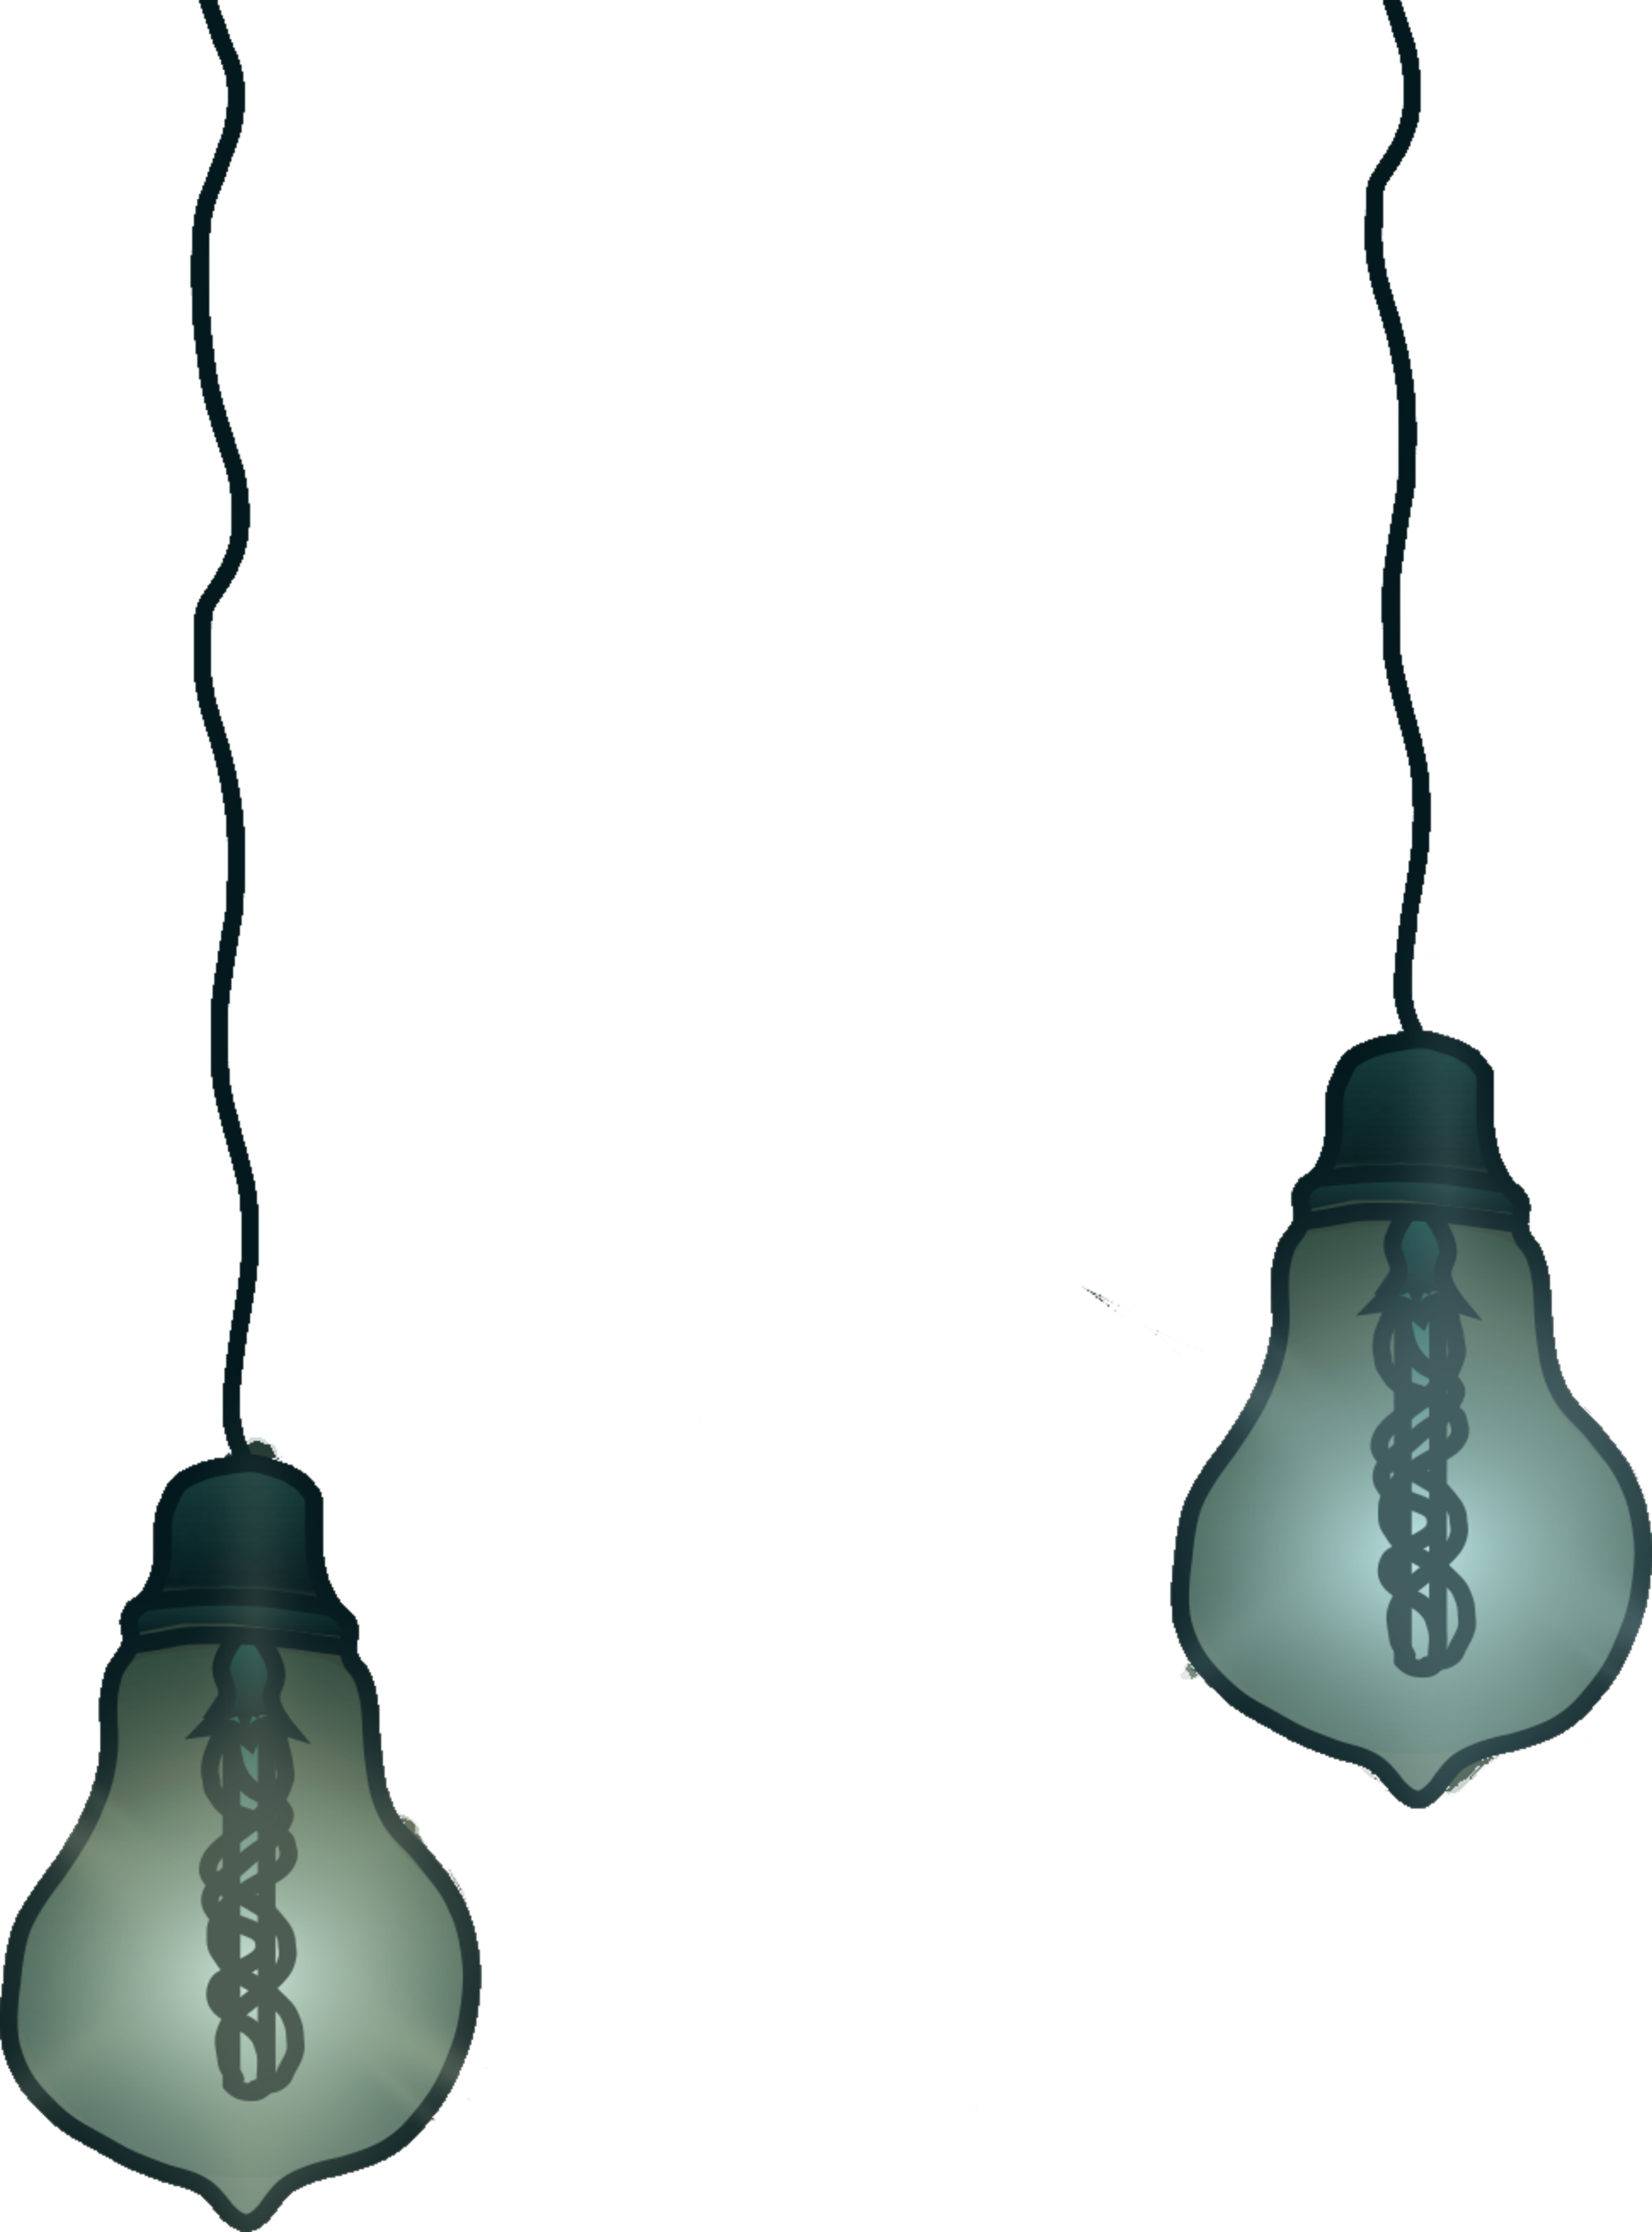
\includegraphics[scale=0.1, angle=0]{zarowki.pdf}
      }
      ;
    \node[yshift=1.0cm,xshift=0.6cm] (logopos) at (current page.south west) {{\begin{tikzpicture}\shuffleducks\duck[signpost=\insertframenumber, \randomhead,scale=.4]\end{tikzpicture}}};
    \pgfmathsetmacro{\progress}{360*(\insertframenumber)/(\inserttotalframenumber)};
    \draw[line width=0.2*3pt] ([xshift=0.55cm] logopos)  arc[radius=0.55cm, start angle=0, end angle=\progress];
    \fill ([shift={(\progress:0.55cm)}] logopos) circle(1pt);

    }
        \end{tikzpicture}
    
}

\newcommand{\SeMPowisko}{%
\large S\normalsize%
\kern-.3em \lower.2ex\hbox{e}%
\lower.2ex\hbox{\large M\normalsize}%
\kern-.1em \raise.1ex\hbox{\large P\normalsize}%
\kern-.3em \lower.2ex\hbox{o}%
\kern-.2em \raise.2ex\hbox{w}%
\lower.2ex\hbox{i}%
s%
\raise.2ex\hbox{k}%
\kern-.3em \lower.2ex\hbox{o}%
}
% \usepackage{microtype}
% \DeclareRobustCommand{\SeMPowisko}{SeMPowisko}


% \newcommand\Tikz{Ti\emph{k}Z}
% \definecolor{neworange}{RGB}{255,140,0}
% \renewcommand{\figurename}{figure}


\title{Alternatywne metody kodowania obrazu}
% \subtitle{Building a Low-Cost Ground Station with SatNOGS}
\author[M. Winiarski]{Mateusz ,,\(\blacksquare\)'' Winiarski}
\institute[Biometria]{biofizyka\(^\dagger\), FAIS, Uniwersytet Jagielloński} 
\date[dzisiaj]{dzisiaj, \today}

\begin{document}

\frame{\titlepage}

\section{Wstęp}

\begin{frame}{~}{}
  \transfade
  \begin{itemize}
    \item \textbf{Kodowanie obrazu} to proces przekształcania danych obrazu w formę, która może być łatwiej przechowywana, przesyłana i przetwarzana
    \item Wykorzystuje różne techniki kompresji, aby zmniejszyć rozmiar pliku obrazu bez znacznej utraty jakości
    \item Istnieją różne metody kodowania obrazu, takie jak JPEG, PNG, GIF, BMP i TIFF
  \end{itemize}

\end{frame}
\begin{frame}{~}{}
  \transfade
  \begin{itemize}
    \item \textbf{JPEG} (Joint Photographic Experts Group) to popularny format kompresji stratnej, który jest szeroko stosowany w fotografii cyfrowej
    \item \textbf{PNG} (Portable Network Graphics) to format bezstratnej kompresji, który obsługuje przezroczystość i jest często używany w grafice internetowej
    \item \textbf{GIF} (Graphics Interchange Format) to format obrazu rastrowego, który obsługuje animacje i jest często używany w mediach społecznościowych
    \item \textbf{BMP} (Bitmap) to format obrazu rastrowego, który przechowuje dane obrazu w postaci pikseli i jest często używany w systemach Windows
    \item \textbf{TIFF} (Tagged Image File Format) to format obrazu bezstratnego, który jest często używany w profesjonalnej fotografii i skanowaniu
  \end{itemize}

  \end{frame}

\begin{frame}{Wprowadzenie}
    \begin{itemize}
        \item JPEG – popularna metoda kodowania obrazu
        \item Cel prezentacji: przedstawienie alternatywnych metod kodowania obrazu – PNG, AVIF i WebP
        \item Różnice w podejściu:
        \begin{itemize}
            \item PNG – bezstratne kodowanie
            \item AVIF i WebP – nowoczesne metody stratne lub hybrydowe
        \end{itemize}
    \end{itemize}
\end{frame}

\begin{frame}{Schemat kodowania obrazu}
  \begin{enumerate}
  \item Przetwarzanie wstępne (przygotowanie danych)

\begin{itemize}
% \item Większość formatów przekształca obraz z \textbf{RGB} (czerwony, zielony, niebieski) do:
\item Konwersja przestrzeni kolorów
  % \begin{itemize}
  % \item 
  {YCbCr}, {CMYK}, {LAB}...
  % \end{itemize}
% \item Powód: Lepsza kompresja (ludzkie oko jest bardziej wrażliwe na jasność niż na kolory)
\item Podpróbkowanie chrominancji (stratne):
% \begin{itemize}
% \item
%  zmniejszenie rozdzielczości kanałów koloru (\textbf{Cb}, \textbf{Cr}), 
 np. z 4:4:4 do 4:2:0 (w JPEG)
% \end{itemize}


% \item Oszczędza miejsce, bo detale kolorów są mniej widoczne
\end{itemize}

\item Kompresja (stratna lub bezstratna)

\begin{itemize}
\item Podział na bloki (np. 8×8 pikseli w JPEG, 16×16 w WebP)
% \item Ułatwia analizę lokalnych wzorców
% \end{itemize}

\item Transformacja matematyczna (dla kompresji stratnej): 
% \begin{itemize}
{DCT} %(Discrete Cosine Transform)
, 
{transformata falkowa}, 
{kwantyzacja}, DST, ADST...
% \end{itemize}

\item Predykcja (dla kompresji bezstratnej):
% \begin{itemize}
filtrowanie linii skanowania 
 zaawansowane modele predykcji
% \end{itemize}

\item Kodowanie entropijne:
% \begin{itemize}
{Huffman (JPEG)},
{kodowanie arytmetyczne (WebP, AVIF)},
{LZW (GIF)}...
\end{itemize}

\item Zapisywanie metadanych i struktury pliku: nagłówek pliku, metadane (EXIF), dane obrazu
% \begin{itemize}
% \item \textbf{Nagłówek pliku}: Informacje o formacie, rozdzielczości, głębi kolorów
% \item \textbf{Metadane}: EXIF (parametry aparatu), ICC (profile kolorów), znaczniki tekstowe
% \item \textbf{Dane obrazu}: Skompresowane bloki + dodatkowe informacje (np. kanał alfa)
% \end{itemize}

\item Optymalizacja (opcjonalnie): dithering, progresywne ładowanie
% \begin{itemize}
% \item \textbf{Dithering}: Symulowanie większej liczby kolorów (np. w GIF)
% \item \textbf{Progresywne ładowanie} (JPEG, WebP): Pokazanie wersji niskiej jakości przed pełnym dekodowaniem
% \end{itemize}
\end{enumerate}
\end{frame}

\section{PNG}


\begin{frame}{PNG – bezstratne kodowanie obrazu}
    \textbf{Filtrowanie przewidywalne}
    \begin{itemize}
        \item Przewidywanie wartości bajtów na podstawie sąsiednich pikseli (lewy, górny, lewy-górny)
        \item Różnica między wartością rzeczywistą a przewidywaną jest kodowana
        \item 5 typów filtrów, wybieranych dla każdej linii obrazu
    \end{itemize}
\end{frame}

\begin{frame}
  \begin{figure}
 \centering
 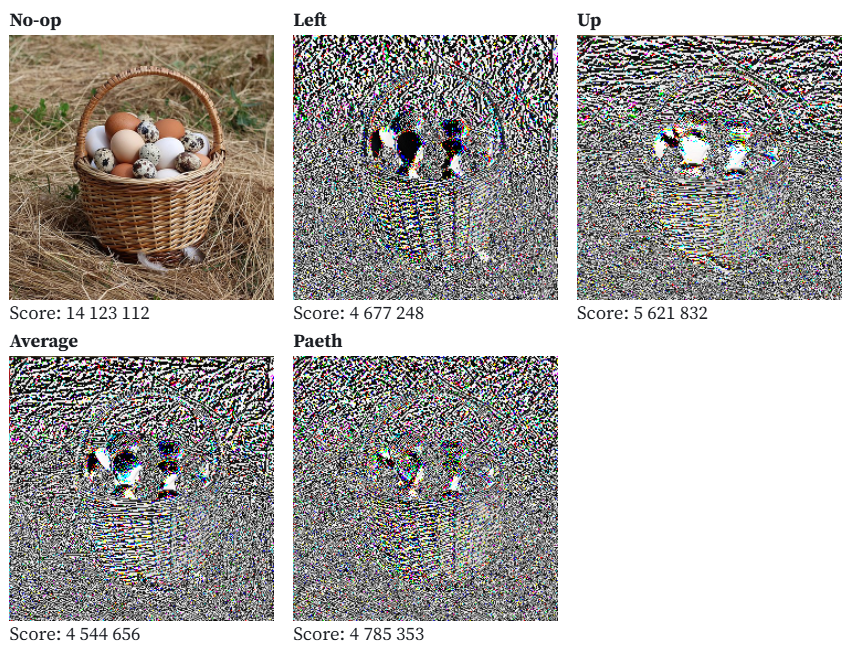
\includegraphics[width=0.7\textwidth]{images/2025-06-13-03-16-22.png}
%  \caption{}
 \end{figure}
\end{frame}

\begin{frame}{PNG – bezstratne kodowanie obrazu (cd.)}
    \textbf{Kompresja Deflate}
    \begin{itemize}
        \item Algorytm Deflate łączy LZ77 i kodowanie Huffmana
        \item Bezstratna kompresja danych po filtrowaniu
    \end{itemize}
    \vspace{0.5cm}
    \textbf{Indeksowane kolory}
    \begin{itemize}
        \item Piksele wskazują na paletę kolorów (zwykle 8-bitową)
        \item Redukcja rozmiaru pliku przy ograniczonej liczbie kolorów
    \end{itemize}
\end{frame}

\begin{frame}{PNG: przeplatanie pikseli}
  \begin{figure}
    \centering
    \foreach \n in {1,...,7} {
    \only<\n>{\includegraphics[width=0.45\textwidth]{images/Adam7_pass_\n.png}\caption{Przeplatanie pikseli: krok \n\ algorytmu Adam7}}
}
  \end{figure}
\end{frame}

% \section{HEIF}
% \begin{frame}{HEIF – applowski format oparty na HEVC}
%     \textbf{HEVC (High Efficiency Video Coding)}
%     \begin{itemize}
%         \item Standard kompresji wideo, znany również jako H.265
%         \item Używa bloków 64x64 pikseli do analizy obrazu
%         \item Wysoka efektywność kompresji w porównaniu do H.264
%     \end{itemize}

%     \end{frame}

% \begin{frame}{HEIF – format oparty na HEVC}
%     \textbf{CABAC (Context-based Adaptive Binary Arithmetic Coding)}
%     \begin{itemize}
%         \item Adaptacyjny kod arytmetyczny
%         \item Dynamiczne dostosowanie modeli prawdopodobieństwa na podstawie kontekstu
%         \item Bardzo efektywna kompresja
%         \item Stosowany w standardzie HEVC, zarówno stratny jak i bezstratny
%     \end{itemize}
% \end{frame}

% \begin{frame}{HEIF cd.}{}
% \begin{figure}
%  \centering
%  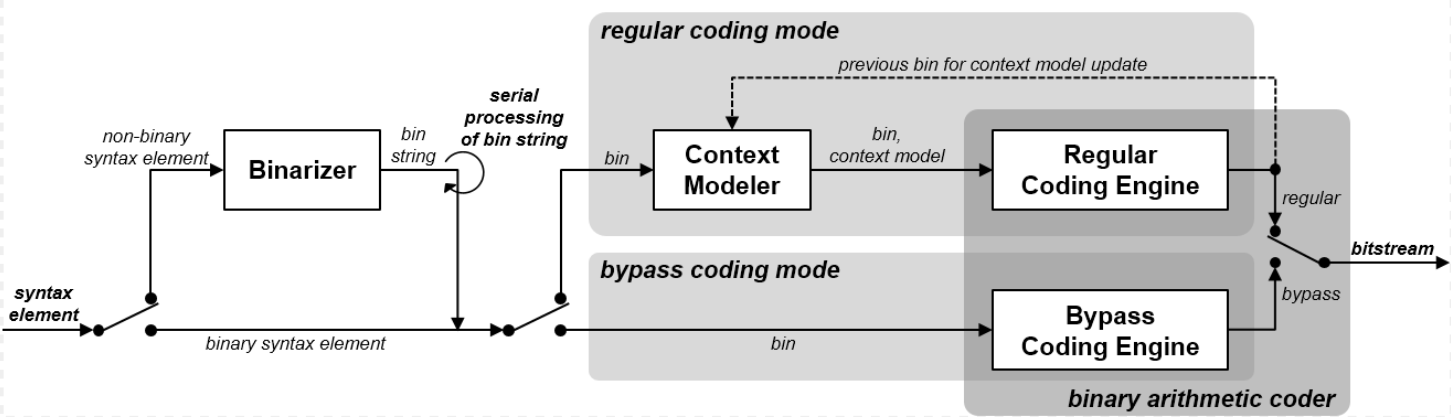
\includegraphics[width=0.7\textwidth]{images/2025-06-13-03-37-32.png}
% %  \caption{}
%  \end{figure}

%  \begin{enumerate}
%   \item \textbf{Binarizacja}  
%     Zamiana każdego symbolu (np. współczynnika transformacji, MV) na ciąg bitów („biny”) zgodnie z regułą (np. Exp‑Golomb, unary) 

%   \item \textbf{Dobór modelu kontekstowego}  
%     Dla każdego bita wybierany jest kontekstowy model prawdopodobieństwa bazujący na uprzednich symbolach (np. L1 normy poprzednich MV) 

%   \item \textbf{Arytmetyczne kodowanie bitu}  
%     Każdy bit kodowany jest przez dzielenie zakresu „range” na podzakresy dla 0 i 1 zgodnie z prawdopodobieństwem z modelu, a następnie wybór jest zakodowany metodą arytmetyczną 

%   \item \textbf{Aktualizacja modelu}  
%     Po zakodowaniu bitu model contextu aktualizuje swoje statystyki (często z „agingiem”), co pozwala adaptacji do lokalnych zmian
% \end{enumerate}
% \end{frame}

\section{WebP}

\begin{frame}{WebP – format stworzony przez Google}
    \begin{itemize}
        \item Wprowadzony w 2010 roku jako alternatywa dla JPEG i PNG
        \item Obsługuje zarówno kompresję stratną, jak i bezstratną
        \item Umożliwia przezroczystość (kanał alfa) i animacje
        \item Szerokie wsparcie w nowoczesnych przeglądarkach
    \end{itemize}
\end{frame}

\begin{frame}{WebP – kompresja stratna}
    \begin{itemize}
        % \item Bazuje na metodach VP8 (intra-frame coding)
        \item Obraz dzielony na makrobloki, które są predykowane na podstawie sąsiadujących bloków
        \item Predykcja redukuje redundancję, pozostawiając mały „residual” do zakodowania
        % \item Residual poddawany jest transformacji DCT, kwantyzacji i kodowaniu entropijnemu (kodowanie arytmetyczne)
        \item Adaptacyjne rozłożenie bitów
        %  – mniej bitów dla segmentów o niskiej entropii, więcej dla skomplikowanych
    \end{itemize}
\begin{figure}
 \centering
 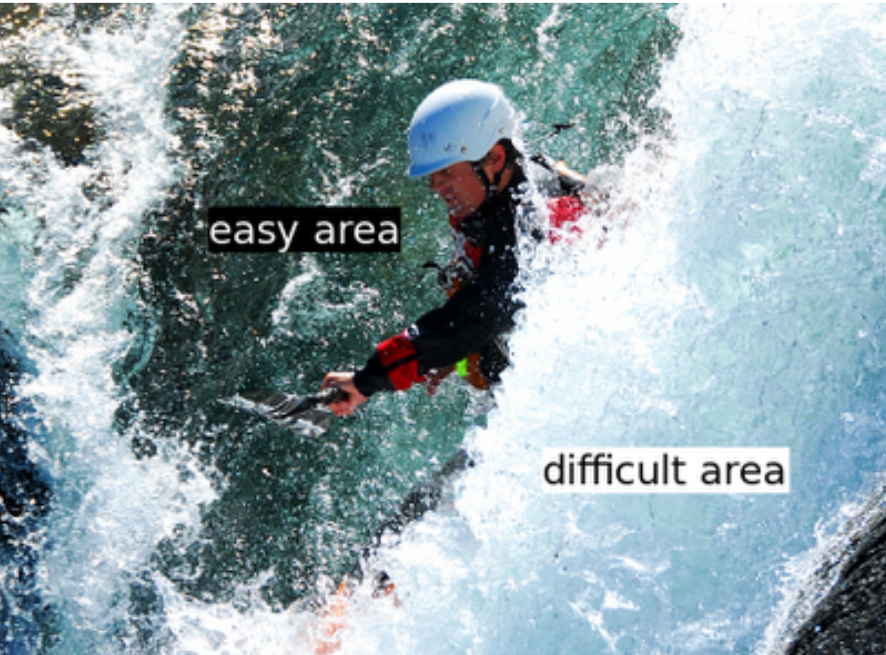
\includegraphics[width=0.4\textwidth]{images/2025-06-13-09-43-35.png}
 \caption{Przykład obszarów ,,łatwych'' i ,,trudnych'' do kompresji w WebP. Standard pozwala na dobieranie parametrów kompresji dla każdego segmentu obrazu.}
 \end{figure}

\end{frame}

\begin{frame}{WebP -- tryby prognozowania}

 \begin{figure}
 \centering
 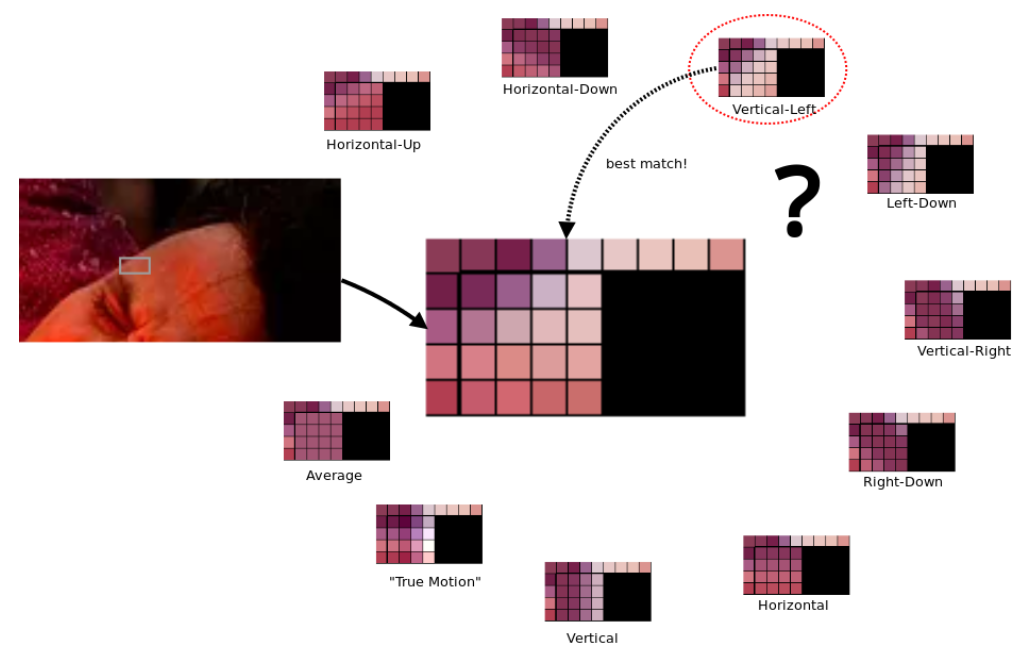
\includegraphics[width=0.8\textwidth]{images/2025-06-13-09-37-42.png}
%  \caption{}
 \end{figure}
\end{frame}

\begin{frame}{WebP – kompresja bezstratna}
    \begin{itemize}
        \item Używa algorytmów LZ77, prefix coding oraz cache kolorów
        \item Zachowuje dokładne wartości pikseli, w tym przezroczystość
        \item Średnio o 25–45\% lepsza kompresja niż PNG
        \item Szybsze dekodowanie niż PNG
    \end{itemize}
    \begin{figure}
 \centering
 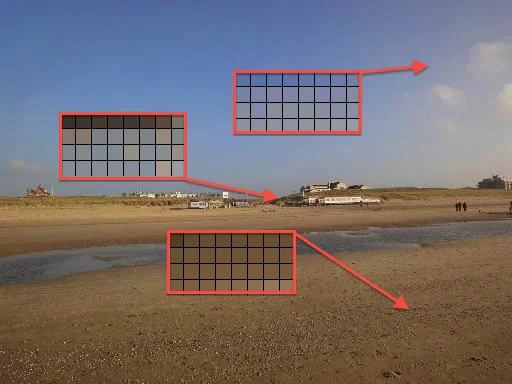
\includegraphics[width=0.4\textwidth]{images/2025-06-13-09-49-42.png}
 \caption{Lokalne palety barw w WebP -- przykład}
 \end{figure}
\end{frame}

\begin{frame}{LZ77 (Lempel-Ziv 1977)}
    % \textbf{LZ77 (Lempel-Ziv 1977)}
    \begin{itemize}
        \item Algorytm kompresji bezstratnej
        \item Wykorzystuje słownik do zastępowania powtarzających się sekwencji znaków
        \item Działa na zasadzie odnajdywania powtórzeń w strumieniu danych
        \item Efektywne kodowanie prefiksem, gdzie dłuższe sekwencje są reprezentowane krótszymi kodami
    \end{itemize}
  \begin{figure}
 \centering
 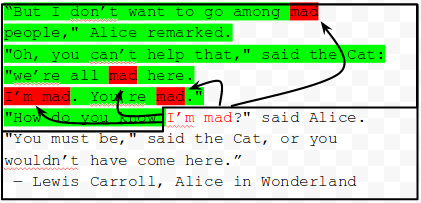
\includegraphics[width=0.7\textwidth]{images/2025-06-13-09-25-53.png}
 \caption{Kodowanie prefiksem LZ77 -- przykład tekstowy}
 \end{figure}
\end{frame}

\begin{frame}{WebP – dodatkowe cechy i opcje kodowania}
    \begin{itemize}
        \item Obsługa kanału alfa w trybach stratnym i bezstratnym
        \item Możliwość animacji (alternatywa dla GIF)
        \item Opcje kodowania: kontrola jakości, filtrowanie, liczba przebiegów, segmentacja, wielowątkowość
        \item Elastyczność w balansowaniu jakości, rozmiaru i szybkości kodowania
    \end{itemize}
\end{frame}

\section{AVIF}

\begin{frame}{AVIF – nowoczesny format oparty na AV1}
    \textbf{Interframe prediction}
    \begin{itemize}
        \item Wykorzystanie informacji z poprzednich i następnych klatek do kompresji (traktowanie obrazu jako filmu)
        \item Redukcja redundancji temporalnej
    \end{itemize}
\end{frame}

\begin{frame}{AVIF – transformaty i kwantyzacja}
    \textbf{DCT vs ADST}
    \begin{itemize}
        \item DCT – klasyczna transformata kosinusowa
        \item ADST – transformata sinusowa asymetryczna, lepsza przy krawędziach
    \end{itemize}
    \vspace{0.5cm}
    \textbf{Kwantyzacja}
    \begin{itemize}
        \item Redukcja informacji mniej istotnych wizualnie
        \item Adaptacyjna i optymalizowana pod kątem jakości i rozmiaru
    \end{itemize}

    \begin{figure}
 \centering
 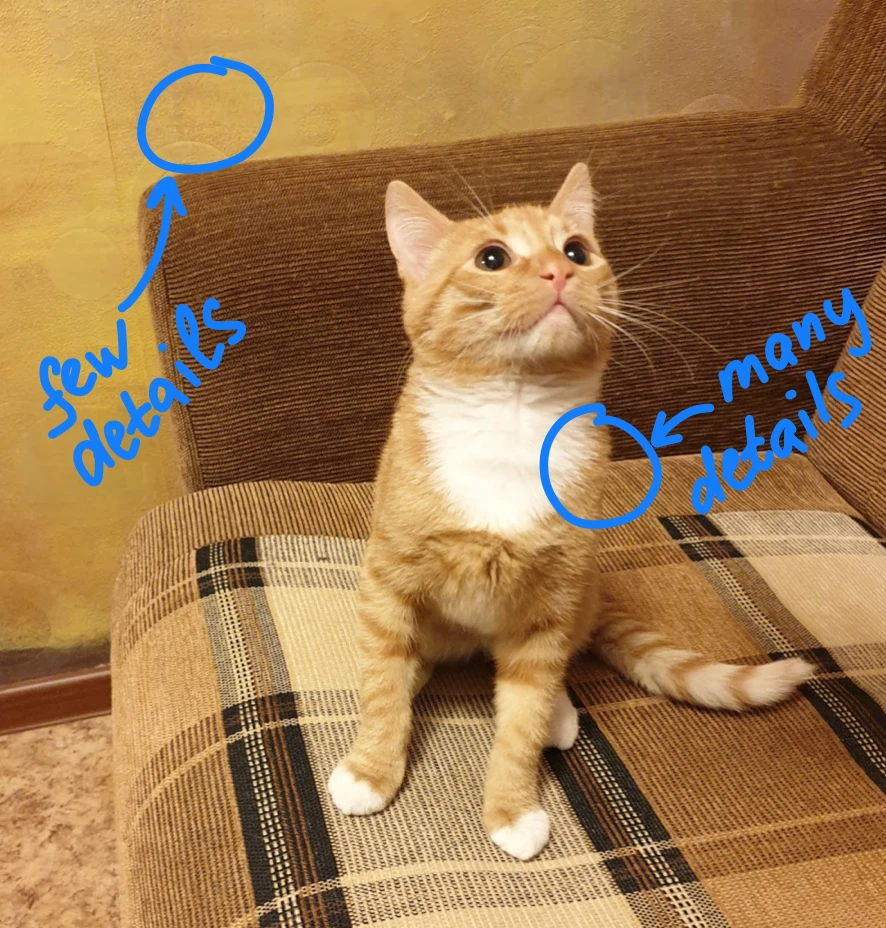
\includegraphics[width=0.3\textwidth]{images/2025-06-13-12-26-02.png}
%  \caption{}
 \end{figure}
\end{frame}

\begin{frame}{AVIF – kodowanie entropijne}
    \begin{itemize}
        \item Adaptacyjne modele prawdopodobieństwa
        \item Efektywne usuwanie redundancji statystycznej
        \item Wysoki stopień kompresji
    \end{itemize}
\end{frame}

\begin{frame}{AVIF: deblocking}
  \begin{figure}
 \centering
 \begin{subfigure}{0.45\textwidth}
 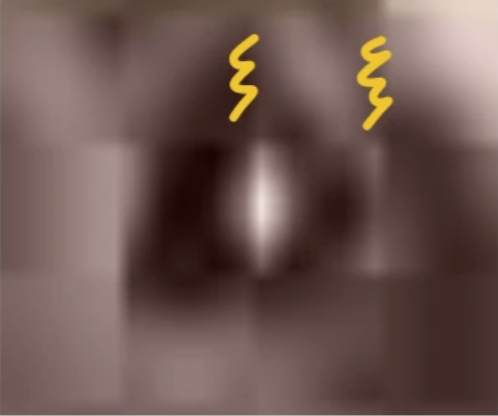
\includegraphics[width=0.9\textwidth]{images/2025-06-13-13-37-14.png}
 \end{subfigure}
 \begin{subfigure}{0.45\textwidth}
 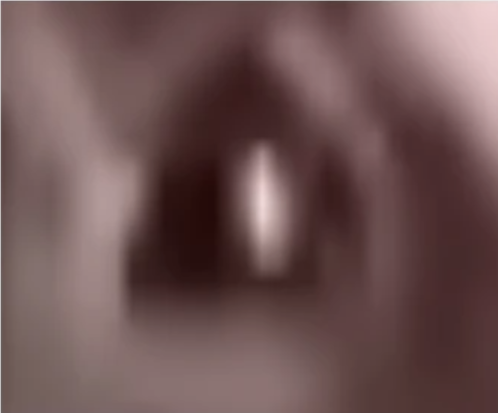
\includegraphics[width=0.9\textwidth]{images/2025-06-13-13-37-59.png}
 \end{subfigure}
 \caption{Próbka obrazu przed i po deblockingu}
 \end{figure}
\end{frame}

\begin{frame}{AVIF: porównanie}
\begin{columns}
  \column{0.5\textwidth}
  \begin{figure}
 \centering
 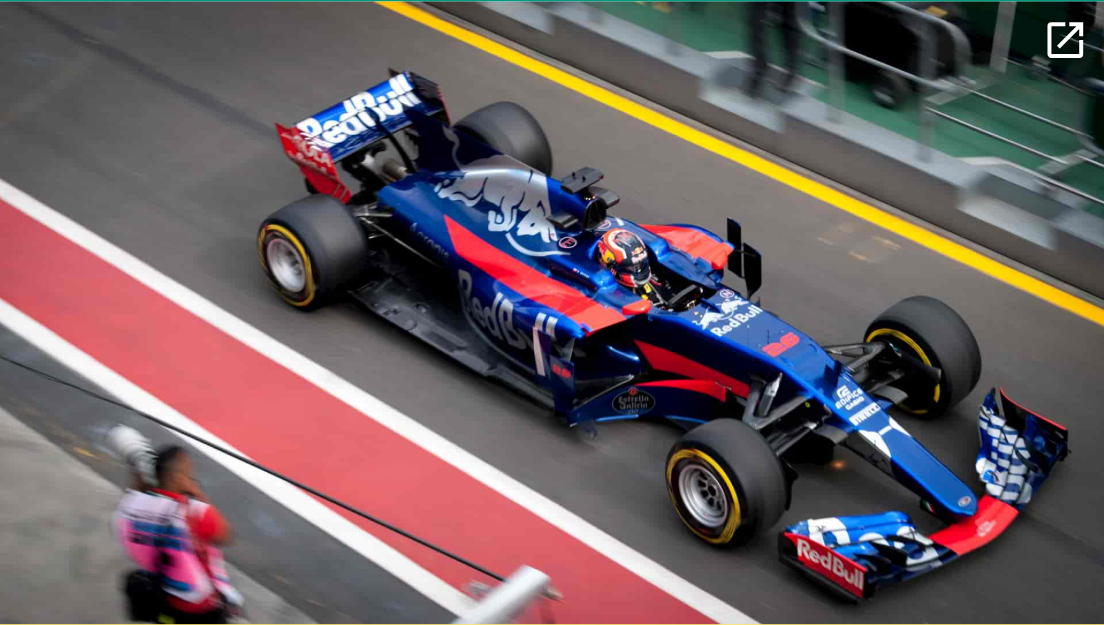
\includegraphics[width=\textwidth]{images/2025-06-13-11-35-46.png}
 \caption{JPEG: 74.4 kB}
 \end{figure}
  \column{0.5\textwidth}
\begin{figure}
 \centering
 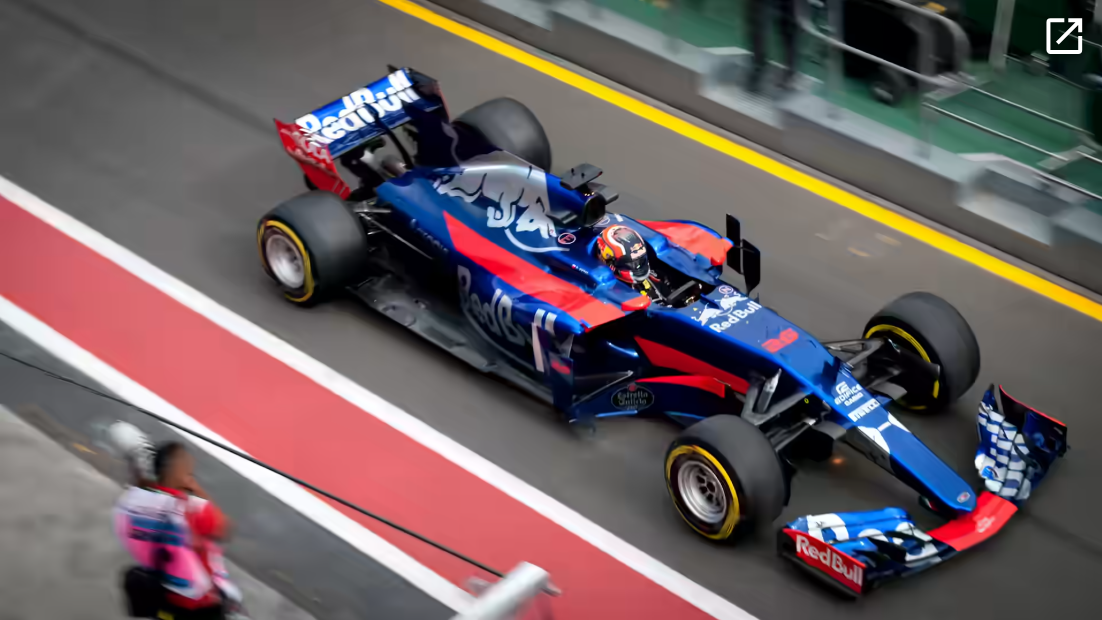
\includegraphics[width=\textwidth]{images/2025-06-13-11-36-20.png}
 \caption{AVIF: 18.2 kB}
 \end{figure}
\end{columns}
\end{frame}

\begin{frame}{AVIF: porównanie}
\begin{columns}
  \column{0.5\textwidth}
\begin{figure}
 \centering
 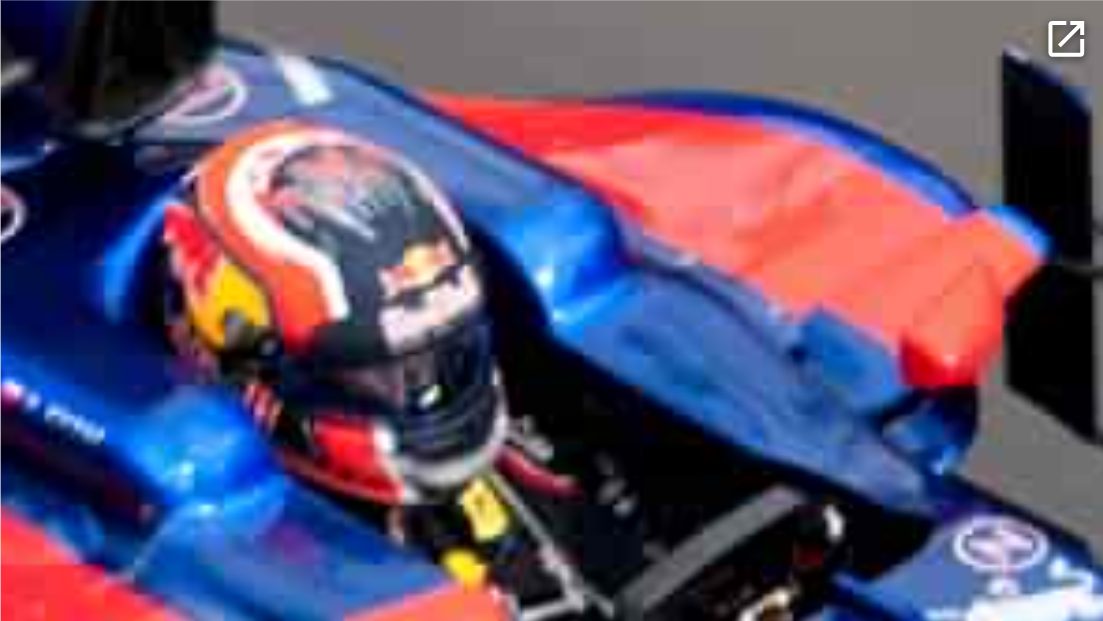
\includegraphics[width=\textwidth]{images/2025-06-13-11-41-43.png}
 \caption{JPEG: 74.4 kB}
 \end{figure}
  \column{0.5\textwidth}
\begin{figure}
 \centering
 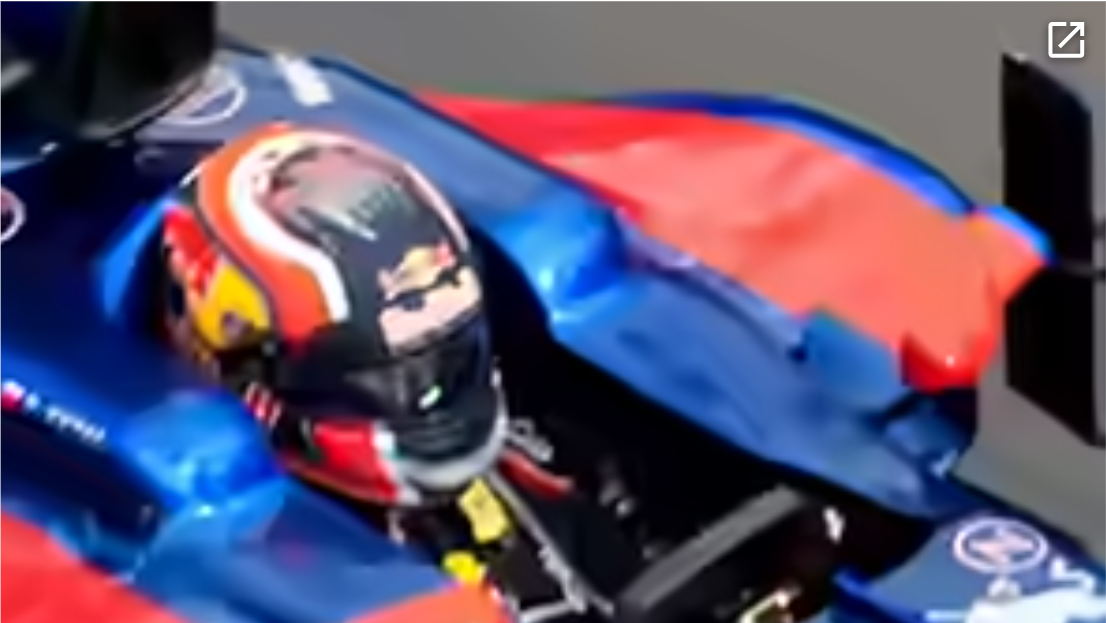
\includegraphics[width=\textwidth]{images/2025-06-13-11-42-03.png}
 \caption{AVIF: 18.2 kB}
 \end{figure}
\end{columns}
\end{frame}

\begin{frame}{AVIF: porównanie}
\begin{columns}
  \column{0.5\textwidth}
\begin{figure}
 \centering
 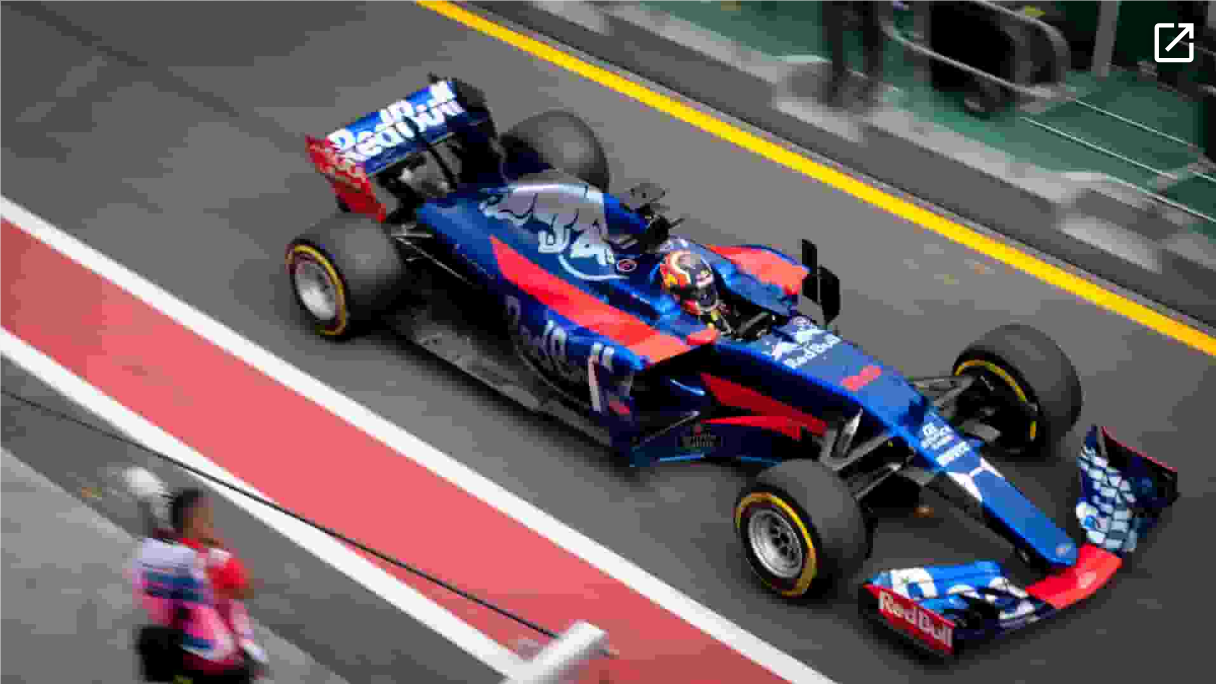
\includegraphics[width=\textwidth]{images/2025-06-13-11-43-24.png}
 \caption{JPEG: 20.7 kB}
 \end{figure}
  \column{0.5\textwidth}
\begin{figure}
 \centering
 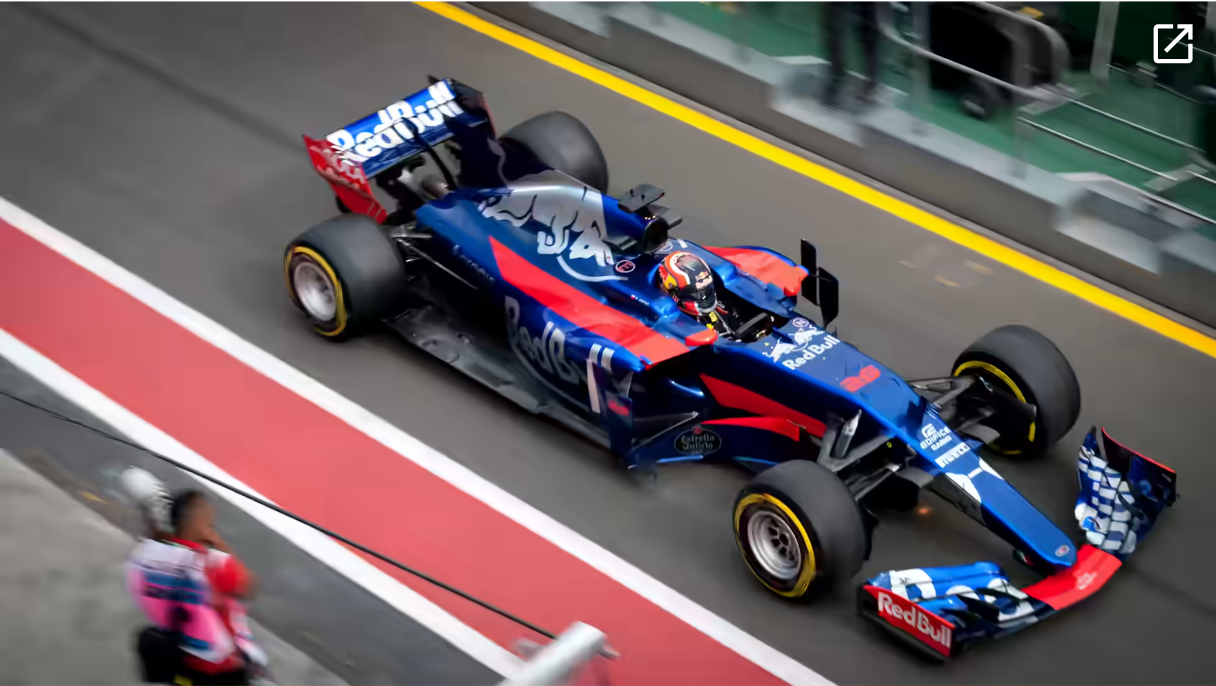
\includegraphics[width=\textwidth]{images/2025-06-13-11-43-43.png}
 \caption{AVIF: 18.2 kB}
 \end{figure}
\end{columns}
\end{frame}

\begin{frame}{AVIF: wady}
  \centering
  \embedvideo{
 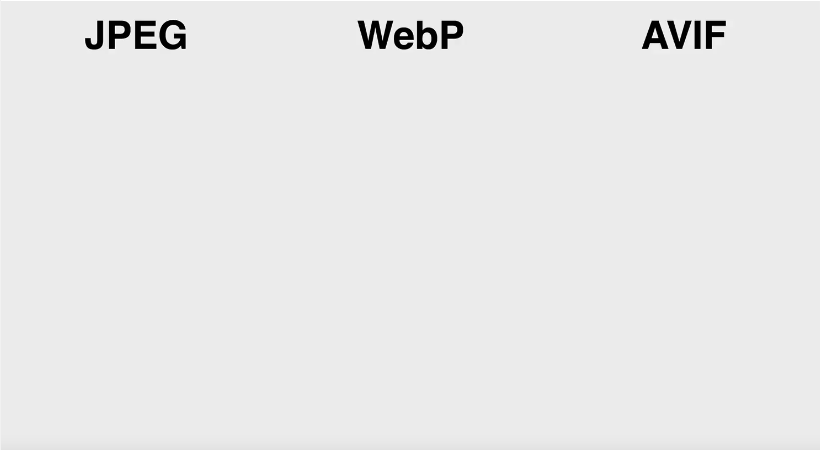
\includegraphics[width=0.8\textwidth]{images/2025-06-13-03-57-05.png}
 }{images/progressive-34922832.mp4}
\end{frame}

\section{Podsumowanie}

\begin{frame}{Podsumowanie}
\begin{figure}
 \centering
 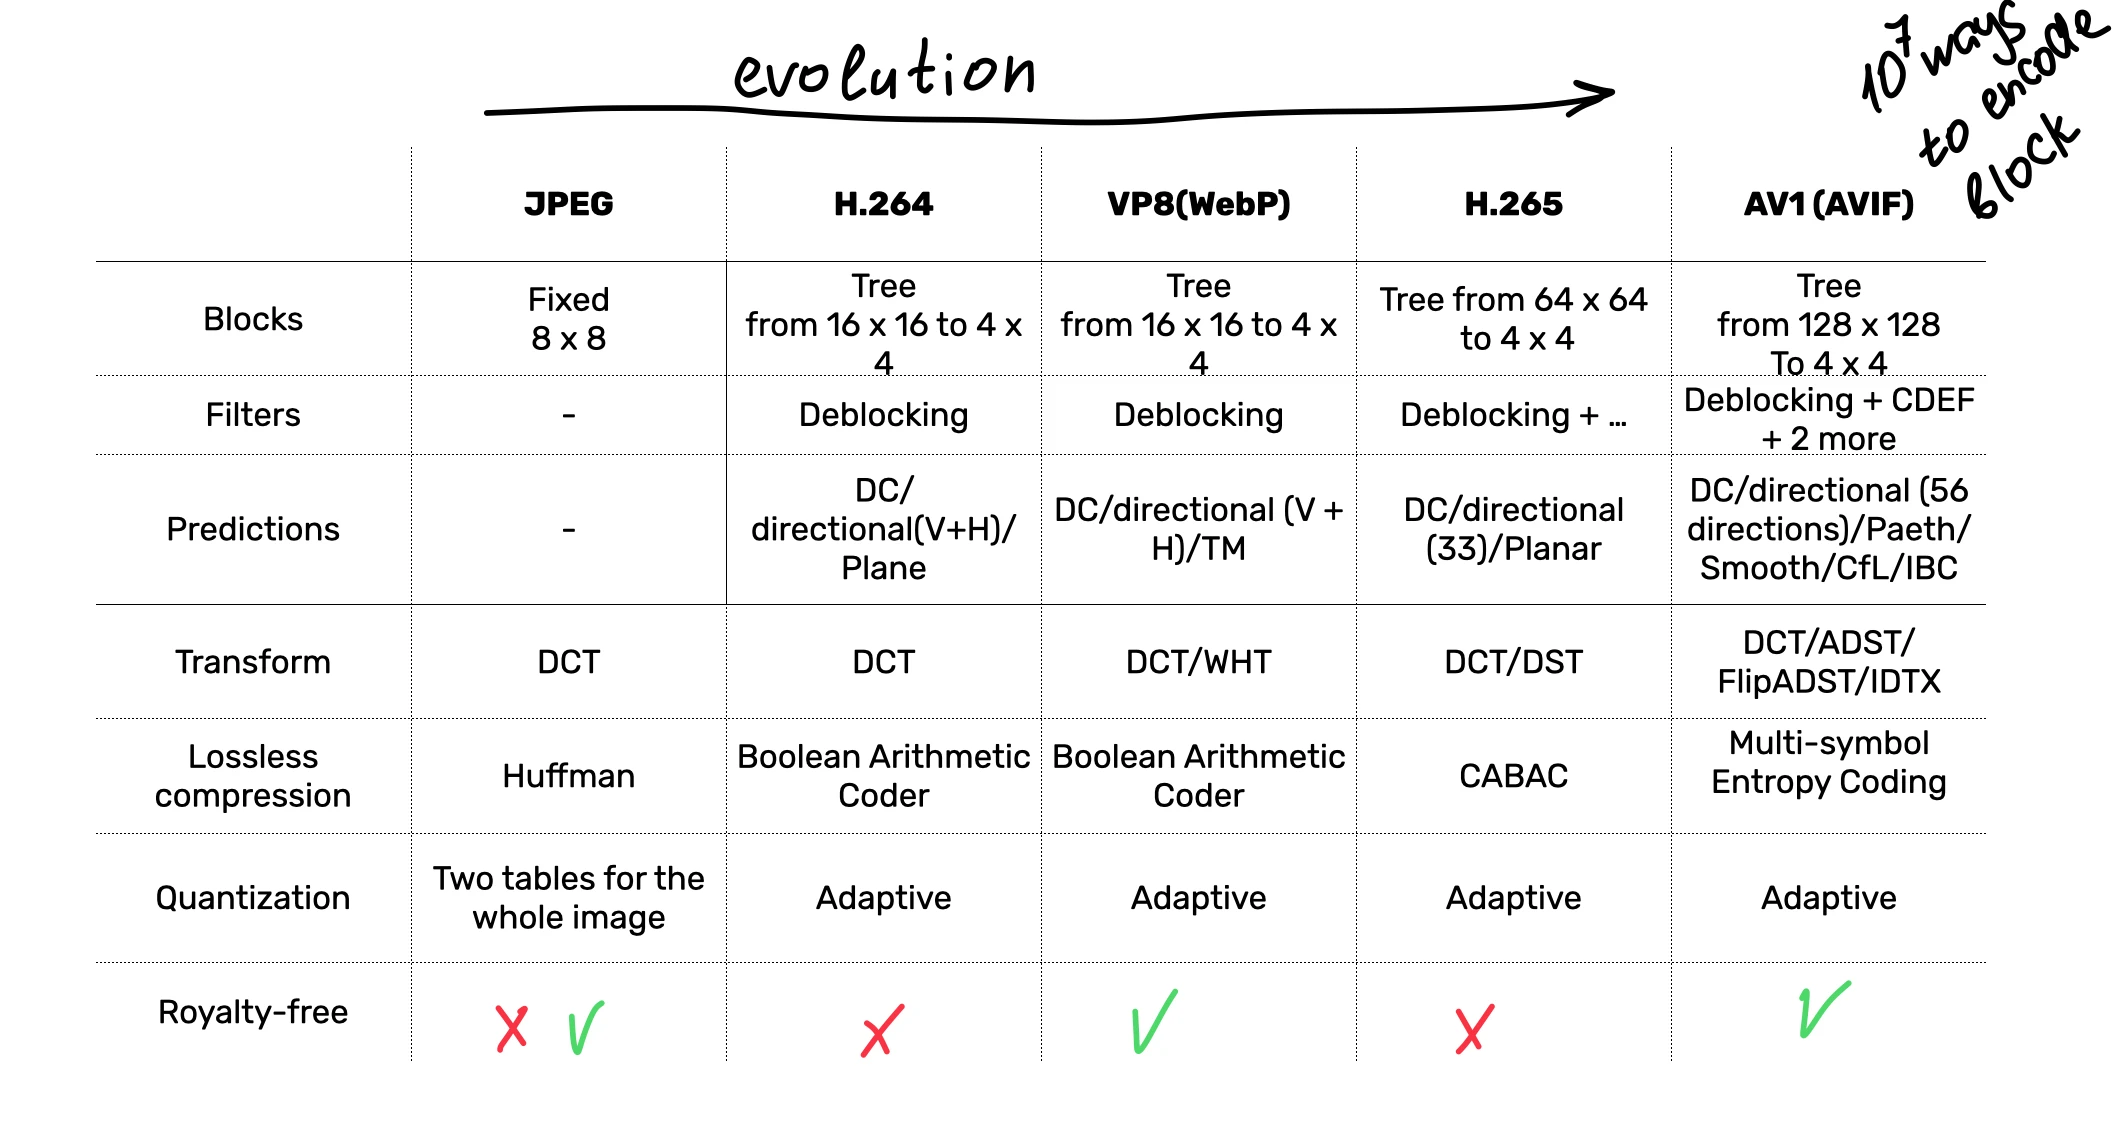
\includegraphics[width=0.9\textwidth]{images/2025-06-13-12-24-32.png}
%  \caption{}
 \end{figure}
\end{frame}

% \begin{frame}{Podsumowanie i porównanie}
%     \begin{tabular}{|l|l|l|}
%         \hline
%         \textbf{Format} & \textbf{Typ kompresji} & \textbf{Kluczowe cechy} \\
%         \hline
%         PNG & Bezstratna & Filtrowanie, Deflate, paleta kolorów \\
%         \hline
%         AVIF & Stratna & Predykcja międzyklatkowa, DCT/ADST, kwantyzacja, kodowanie entropijne \\
%         \hline
%         HEIF & Stratna/bezstratna & CABAC, oparty na HEVC, wysoka kompresja \\
%         \hline
%     \end{tabular}
% \end{frame}

% \section{~}

\begin{frame}{Bibliografia}{}
  \nocite{*}
  \printbibliography[heading=none]
\end{frame}


\begin{frame}{~}{}
  \transglitter
  \vspace{-1cm}
\begin{figure}
\centering
  \begin{tikzpicture}
    \duck[parrot, body=gray!30!yellow, head=gray!30!yellow, bill=red, torch=gray!70!brown, tshirt=blue!40!black, ribbon=gray, bowtie=blue!50!white, crazyhair=black]
    %\addwater{blue!50!cyan}
    \fill[cyan!20!white] (-1.4,1.8) ellipse (1.8 and 0.5);
\fill[cyan!20!white] (-0.2,1.54) -- (0.2,1.35) -- (0.0,1.6) -- cycle;
\node at (-1.4,1.8) {dziękuję za uwagę};
  \end{tikzpicture}
  \end{figure}


  
  \begin{figure}
  \centering
        % 
\includegraphics[height=0.3\linewidth]{images/2025-05-13-15-25-41.png}\\
      \qrcode[height=0.3\textwidth]{https://github.com/falcotinnunculus/przezrocza/blob/wladca/biometri/l.pdf}
  {\scriptsize \url{https://github.com/falcotinnunculus/przezrocza/blob/wladca/biometri/l.pdf}}

  \end{figure}
% \vspace{-5.3cm}
% \transparent{0.7}
  % \begin{figure}
      % \centering
      % \caption{Caption}
      % \label{fig:enter-label}
  % \end{figure}
\end{frame}

\end{document}